\documentclass[main.tex]{subfiles}
\begin{document}

\section{Draw a circuit to control a green LED at 10mA current from a microcontroller GPIO pin capable of sourcing and sinking 5mA maximum with a 3.3V logic level?}

\spoilerline
\subsection{Context}
Discrete LEDs (\textit{Light Emitting Diodes}) are often used on circuit boards indicators to end users and firmware developers about the state of an embedded system\footnote{LEDs can also be a primary feature of a device - an example case is high power LEDs, such as automobile headlights, which require more complex circuitry to drive. This question will address only the simpler case of lower power LEDs.}. A common first program executed during board bring-up by firmware developers is to blink the onboard LEDs as an indicator the microcontroller is alive and functional. For end users, it is very common to use LEDs to indicate that the embedded system is powered on and operating nominally. Often, in electronic circuits, an LED is connected in some fashion to a microcontroller GPIO (\textit{General Purpose Input / Output}) pin in order to turn it on and off via firmware. 

\subsection{Controlling Current to an LED} 
\noindent The circuit given in figure \ref{fig:led_circuit_simple} shows a simple schematic of an LED powered from a constant voltage source, $V_s$, with a fixed resistance, $R_l$ in series with the LED. The LED has a forward voltage drop, $V_f$, and a forward current, $I_f$. The goal is to determine the value of $R_l$, limiting the current through the LED ($I_f$).

\begin{figure}[h!]
    \begin{center}
        \begin{circuitikz}[american]
            \draw (0, 6) node[vcc] () {$V_s$};
            \draw (0, 6) to[empty led, v=$V_f$, i=$I_f$] (0, 4);
            \draw (0, 4) to[resistor, l=$R_l$] (0, 2);
            \draw (0, 2) node[ground] () {};
            \label{fig:led_circuit_simple}
        \end{circuitikz}
        \caption{Voltage Source Powering an LED}
    \end{center}
\end{figure}

\noindent The circuit can be solved by modelling the forward voltage drop of the LED, $V_f$, as a fixed voltage and applying Ohms Law to solve for solve for $R_l$, as shown in equation \eqref{eq:led_current_limitting_resistor_math}:

\begin{equation}
    \begin{aligned}[b]
        V_s - V_f &= R_l \cdot I _f \\
        R_l &= \frac{V_s - V_f}{I_f}
    \end{aligned}
    \label{eq:led_current_limitting_resistor_math}
\end{equation}

\noindent Note that for LEDs, the brightness is proportional to the current flowing through the LED. Consequently, the brightness of the LED can be varied by changing the resistance value or the voltage to the LED\footnote{To give a reference, small 0603 LEDs are usually rated for 20mA max (so 20mA * 2V = 40mW), and are visible indoors at just 1mA. For a firmware debugging LED, ~2.5mA, is very common}. In practice, an LED's forward voltage is somewhat dependent on $I_f$ and device temperature. "I-V Curves" across temperature are usually given by LED manufacturers in the LED's datasheets, however, an assumption of a constant $V_f$ is enough for approximate solutions.

\subsection{Transistors}
Transistors are three terminal, electronically-controlled switches in which one terminal is used to control the switching between the other two terminals. The two most commonly used transistors are MOSFETs (\textit{Metal Oxide Semiconductor Field Effect Transistors}) and BJTs (\textit{Bipolar Junction Transistors}), though there are other types. For a BJT, a small current to the base allows a large current to flow between emitter and collector terminals. For a FET (\textit{Field Effect Transistor}), a voltage potential difference between the gate and the source allows current to flow between drain and source. These devices can be drawn with a variety of schematic symbols, but are most commonly seen as:

\begin{figure}[H]
    \begin{center}
        \begin{circuitikz}[american]
            \draw (0, 4) node[npn] (q1) {NPN BJT};
            \draw (q1.E) ++ (0, -0.5) node[anchor=south]{Emitter};
            \draw (q1.B) ++ (-1, 0) node[anchor=west]{Base};
            \draw (q1.C) ++ (0, 0.5) node[anchor=north]{Collector};
            \draw (4, 4) node[pnp] (q2) {PNP BJT};
            \draw (q2.E) ++ (0, 0.5) node[anchor=north]{Emitter};
            \draw (q2.B) ++ (-1, 0) node[anchor=west]{Base};
            \draw (q2.C) ++ (0, -0.5) node[anchor=south]{Collector};
            \draw (8, 4) node[nigfete](q3){NCH FET};
            \draw (q3.G) ++ (-1, 0) node[anchor=west]{Gate};
            \draw (q3.S) ++ (0, -0.5) node[anchor=south]{Source};
            \draw (q3.D) ++ (0, 0.5) node[anchor=north]{Drain};
            \draw(12, 4) node[pigfete](q4){PCH FET};
            \draw (q4.G) ++ (-1, 0) node[anchor=west]{Gate};
            \draw (q4.D) ++ (0, -0.5) node[anchor=south]{Drain};
            \draw (q4.S) ++ (0, 0.5) node[anchor=north]{Source};
            \label{fig:transistors}
        \end{circuitikz}
        \caption{Common Transistors}
    \end{center}
\end{figure}

\noindent FET's, ideally, do not require any power consumption to keep them enabled, whereas BJTs require current to be supplied constantly. This means FETs are typically preferred when power consumption is a critical consideration; this is primarily for higher power circuits in which excessive power consumption directly results in a need for expensive cooling systems. BJTs are a much older technology and are easier to fabricate, making them far preferred when optimizing for cost. \newline

\newnoindentpara Another consideration is low versus high side switching when using a transistor to enable and disable (aka switch) a load. The solution presented in figure \ref{fig:led_circuit} demonstrates low side switching. There are numerous implications of this design decision. % maybe add a quick one-liner

% Don't want to do any more drawings or open to can of worms too much here, hopefully this is sufficient? Could even scope creep and add a new question "Would you use high side or low side switch for this load.

% Removed Content
% When switching high current loads, NCH FETs are preferred because they have lower RDSon (\textit{Resistance Drain-Source when On}) and therefore lower conduction losses than PCH FETs. To turn an NCH FET a positive voltage must be generated between the gate and the source, $V_{gs} > 0$. 

% References
% https://www.elektormagazine.com/articles/high-side-low-side-switching
% https://www.baldengineer.com/low-side-vs-high-side-transistor-switch.html

\subsection{Controlling the LED from a Microcontroller} 

\noindent From the question, it's given that the microcontroller GPIO (\textit{General Purpose Input / Output}) pin is not capable of providing enough current to drive the LED (\textit{Light Emitting Diode}) as desired. As a result, an external transistor can be used to buffer the control signal from the microcontroller, but draw the current from another voltage source that can supply the required current. The following circuit in figure \ref{fig:led_circuit} demonstrates a simple, cost optimized solution to this problem using a BJT.

\begin{figure}[H]
    \begin{center}
        \begin{circuitikz}[american]
            \draw (0, 6) node[vcc] () {$+3.3V$};
            \draw (0, 6) to[empty led] (0, 4.5);
            \draw (0, 4.5) to[resistor, l=$R_l$] (0, 3);
            \draw (0, 3) -- (0, 2.5);
            \draw (0, 2) node[npn, xscale=-1] (q1) {};
            \draw (q1.E) node[ground]{};
            \draw (q1.B) to[resistor, l=$R_b$] ++ (2.2, 0);
            \draw[thick] (3, 3) rectangle (5, 1) node[pos=0.5]{GPIO};;
            \label{fig:led_circuit}
        \end{circuitikz}
        \caption{GPIO driving an LED}
    \end{center}
\end{figure}

\noindent The base resistor, $R_b$ can be sized to a low E-series value (\textasciitilde $100 \ \Omega$). The forward voltage drop of a green LED, $V_f$, is roughly $2V$ - equation \eqref{eq:led_current_limitting_resistor} can be used to solve for $R_l$. This resistor can be found in the E24 resistor series as a common resistor value so no rounding is needed. % I feel like the E24 comment should be a footnote to avoid confusing a potential reader, or elaborated upon to make it more clear if E-series is a key concept to understand the solution.

% @daniel can't you go a lot lower on the BJT than 100 ohms? I_b = Beta * I_c. Assuming a 3.3V pin and 0.7 Vbe, I_b = (3.3 - 0.7) / 100 = 26 mA, exceeding the 10mA from the pin...
% @ daniel I've been asked to walk thru the BJT math, might be helpful since the 100 ohms is given without explanation or intuition about why it's chosen. Think that is a natural follow-up from the transistor section, and it's a good opportunity to show how to calculate the base resistor value.

\begin{equation}
    R_l = \frac{V_s - V_f}{I_f} = \frac{3.3-2}{10\,\text{mA}} = 130 \,\Omega
    \label{eq:led_current_limitting_resistor}
\end{equation}


\subsection{Pulse Width Modulation}
When controlling an LED from a microcontroller, the brightness of the LED can be modulated using PWM (\textit{Pulse Width Modulation}). Adjusting the \textit{duty cycle} (amount of 'on' or logic high time) of pulse width modulation, provided the frequency $f$ is much greater than perceivable by the human eye, results in the appearance that the LED brightness is changing. If $f$ is too low then it will be apparent to a viewer that the LED is turning on and off. PWM implementations are usually done in hardware via dedicated timers, where the frequency is set to a constant, high value and the timer's duty cycle is adjusted to control the brightness. An example of a PWM waveform with a duty cycle of 80\% is shown in figure \ref{fig:pwm_waveform}.

\begin{figure}[H]
    \centering
    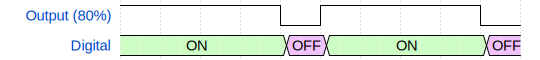
\includegraphics[scale=0.4]{generated_images/svg_generated/pwm.png}
    \caption{PWM Waveform}
    \label{fig:pwm_waveform}
\end{figure}

\noindent Note that PWM's application is not limited to LEDs - in general, PWM can be thought of as a way to control the average voltage across a load, and is used in motor control, power supplies, and more.

\end{document}
